\documentclass{standalone}
\usepackage{tikz}
\usetikzlibrary{patterns, positioning}


\begin{document}
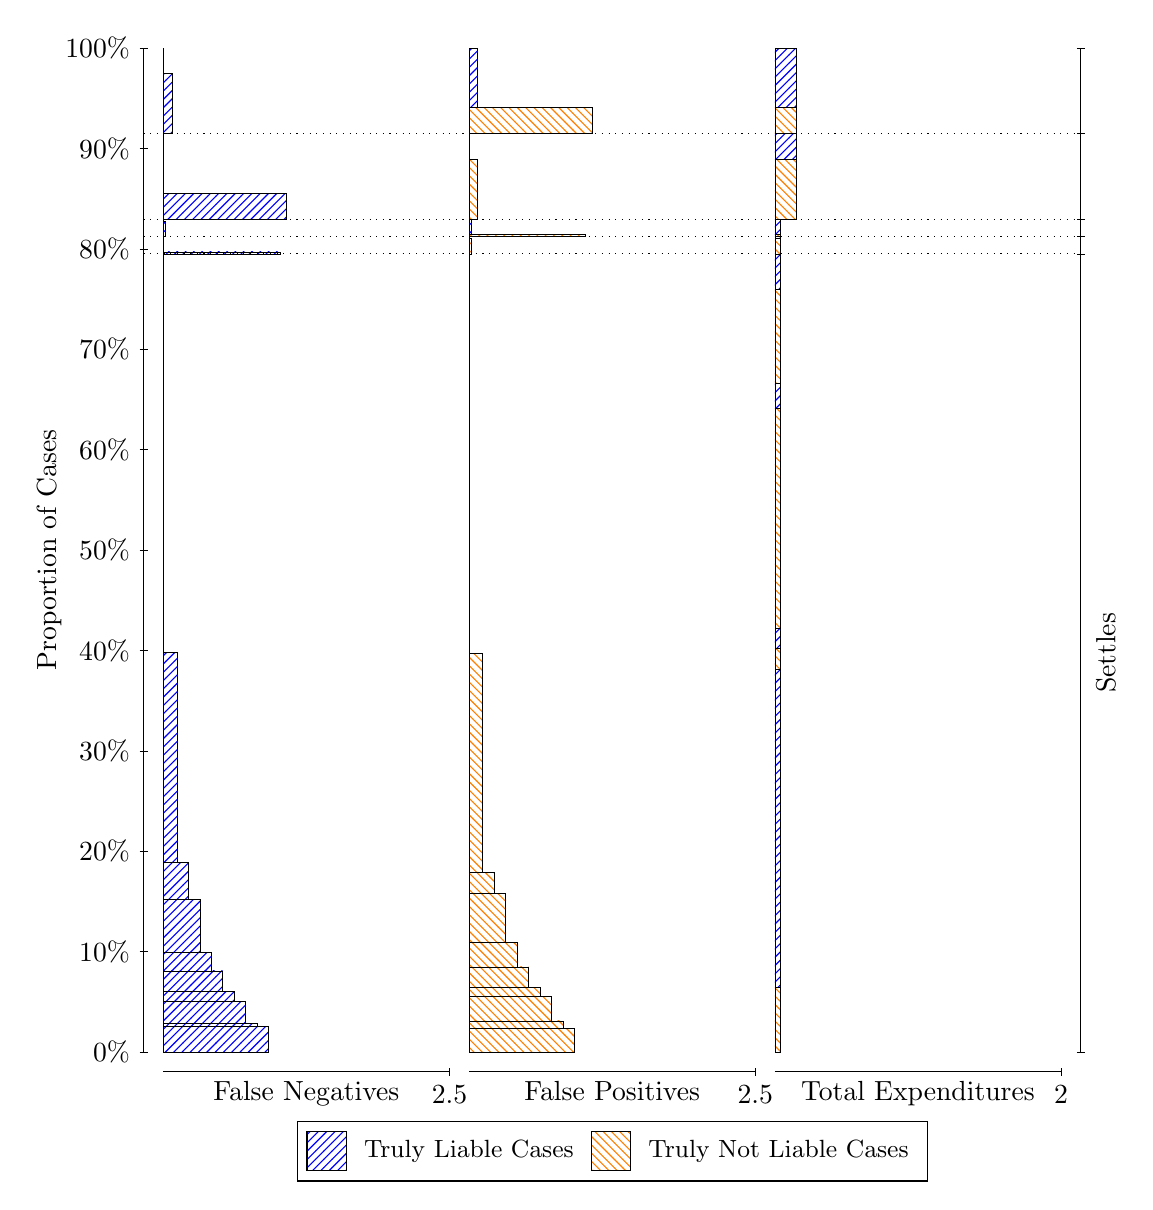
\begin{tikzpicture}
\draw[black, very thin] (1.5,1.75) -- (1.5,14.5);
\node[rotate=90, text=black, anchor=center] at (0.3, 8.125) {Proportion of Cases};
\draw[black, very thin] (1.45,1.75) -- (1.55,1.75);
\node[text=black, anchor=east] at (1.45, 1.75) {0\%};
\draw[black, very thin] (1.45,3.025) -- (1.55,3.025);
\node[text=black, anchor=east] at (1.45, 3.025) {10\%};
\draw[black, very thin] (1.45,4.3) -- (1.55,4.3);
\node[text=black, anchor=east] at (1.45, 4.3) {20\%};
\draw[black, very thin] (1.45,5.575) -- (1.55,5.575);
\node[text=black, anchor=east] at (1.45, 5.575) {30\%};
\draw[black, very thin] (1.45,6.85) -- (1.55,6.85);
\node[text=black, anchor=east] at (1.45, 6.85) {40\%};
\draw[black, very thin] (1.45,8.125) -- (1.55,8.125);
\node[text=black, anchor=east] at (1.45, 8.125) {50\%};
\draw[black, very thin] (1.45,9.4) -- (1.55,9.4);
\node[text=black, anchor=east] at (1.45, 9.4) {60\%};
\draw[black, very thin] (1.45,10.675) -- (1.55,10.675);
\node[text=black, anchor=east] at (1.45, 10.675) {70\%};
\draw[black, very thin] (1.45,11.95) -- (1.55,11.95);
\node[text=black, anchor=east] at (1.45, 11.95) {80\%};
\draw[black, very thin] (1.45,13.225) -- (1.55,13.225);
\node[text=black, anchor=east] at (1.45, 13.225) {90\%};
\draw[black, very thin] (1.45,14.5) -- (1.55,14.5);
\node[text=black, anchor=east] at (1.45, 14.5) {100\%};

\draw[black, very thin] (13.4,1.75) -- (13.4,14.5);
\draw[black, very thin] (13.35,1.75) -- (13.45,1.75);
\node[anchor=west] at (13.35, 1.75) {};
\draw[black, very thin] (13.35,11.886) -- (13.45,11.886);
\node[anchor=west] at (13.35, 11.886) {};
\draw[black, very thin] (13.35,12.105) -- (13.45,12.105);
\node[anchor=west] at (13.35, 12.105) {};
\draw[black, very thin] (13.35,12.325) -- (13.45,12.325);
\node[anchor=west] at (13.35, 12.325) {};
\draw[black, very thin] (13.35,13.416) -- (13.45,13.416);
\node[anchor=west] at (13.35, 13.416) {};
\draw[black, very thin] (13.35,14.5) -- (13.45,14.5);
\node[anchor=west] at (13.35, 14.5) {};

\draw[black, very thin, pattern color=blue, pattern=north east lines] (1.75,1.75) rectangle (3.0852,2.0747);
\draw[black, very thin, pattern color=blue, pattern=north east lines] (1.75,2.0747) rectangle (2.9399,2.1179);
\draw[black, very thin, pattern color=blue, pattern=north east lines] (1.75,2.1179) rectangle (2.7946,2.3907);
\draw[black, very thin, pattern color=blue, pattern=north east lines] (1.75,2.3907) rectangle (2.6492,2.5205);
\draw[black, very thin, pattern color=blue, pattern=north east lines] (1.75,2.5205) rectangle (2.5039,2.7792);
\draw[black, very thin, pattern color=blue, pattern=north east lines] (1.75,2.7792) rectangle (2.3586,3.0171);
\draw[black, very thin, pattern color=blue, pattern=north east lines] (1.75,3.0171) rectangle (2.2133,3.692);
\draw[black, very thin, pattern color=blue, pattern=north east lines] (1.75,3.692) rectangle (2.0679,4.1547);
\draw[black, very thin, pattern color=blue, pattern=north east lines] (1.75,4.1547) rectangle (1.9226,6.8218);
\draw[black, very thin, pattern color=orange, pattern=north west lines] (1.75,6.8218) rectangle (1.75,11.886);
\draw[black, very thin, pattern color=blue, pattern=north east lines] (1.75,11.886) rectangle (3.2306,11.91);
\draw[black, very thin, pattern color=orange, pattern=north west lines] (1.75,11.91) rectangle (1.75,12.105);
\draw[black, very thin, pattern color=blue, pattern=north east lines] (1.75,12.105) rectangle (1.7773,12.3);
\draw[black, very thin, pattern color=orange, pattern=north west lines] (1.75,12.3) rectangle (1.75,12.325);
\draw[black, very thin, pattern color=blue, pattern=north east lines] (1.75,12.325) rectangle (3.3123,12.652);
\draw[black, very thin, pattern color=orange, pattern=north west lines] (1.75,12.652) rectangle (1.75,13.416);
\draw[black, very thin, pattern color=blue, pattern=north east lines] (1.75,13.416) rectangle (1.859,14.173);
\draw[black, very thin, pattern color=orange, pattern=north west lines] (1.75,14.173) rectangle (1.75,14.5);
\draw[black, very thin, pattern color=orange, pattern=north west lines] (5.6333,1.75) rectangle (6.9686,2.051);
\draw[black, very thin, pattern color=orange, pattern=north west lines] (5.6333,2.051) rectangle (6.8233,2.1453);
\draw[black, very thin, pattern color=orange, pattern=north west lines] (5.6333,2.1453) rectangle (6.6779,2.4557);
\draw[black, very thin, pattern color=orange, pattern=north west lines] (5.6333,2.4557) rectangle (6.5326,2.5721);
\draw[black, very thin, pattern color=orange, pattern=north west lines] (5.6333,2.5721) rectangle (6.3873,2.8307);
\draw[black, very thin, pattern color=orange, pattern=north west lines] (5.6333,2.8307) rectangle (6.2419,3.1421);
\draw[black, very thin, pattern color=orange, pattern=north west lines] (5.6333,3.1421) rectangle (6.0966,3.7627);
\draw[black, very thin, pattern color=orange, pattern=north west lines] (5.6333,3.7627) rectangle (5.9513,4.0272);
\draw[black, very thin, pattern color=orange, pattern=north west lines] (5.6333,4.0272) rectangle (5.8059,6.8145);
\draw[black, very thin, pattern color=blue, pattern=north east lines] (5.6333,6.8145) rectangle (5.6333,11.886);
\draw[black, very thin, pattern color=orange, pattern=north west lines] (5.6333,11.886) rectangle (5.6606,12.081);
\draw[black, very thin, pattern color=blue, pattern=north east lines] (5.6333,12.081) rectangle (5.6333,12.105);
\draw[black, very thin, pattern color=orange, pattern=north west lines] (5.6333,12.105) rectangle (7.1139,12.13);
\draw[black, very thin, pattern color=blue, pattern=north east lines] (5.6333,12.13) rectangle (5.6606,12.325);
\draw[black, very thin, pattern color=orange, pattern=north west lines] (5.6333,12.325) rectangle (5.7423,13.089);
\draw[black, very thin, pattern color=blue, pattern=north east lines] (5.6333,13.089) rectangle (5.6333,13.416);
\draw[black, very thin, pattern color=orange, pattern=north west lines] (5.6333,13.416) rectangle (7.1957,13.743);
\draw[black, very thin, pattern color=blue, pattern=north east lines] (5.6333,13.743) rectangle (5.7423,14.5);
\draw[black, very thin, pattern color=orange, pattern=north west lines] (9.5167,1.75) rectangle (9.5848,2.5721);
\draw[black, very thin, pattern color=blue, pattern=north east lines] (9.5167,2.5721) rectangle (9.5848,6.6147);
\draw[black, very thin, pattern color=orange, pattern=north west lines] (9.5167,6.6147) rectangle (9.5848,6.8733);
\draw[black, very thin, pattern color=blue, pattern=north east lines] (9.5167,6.8733) rectangle (9.5848,7.132);
\draw[black, very thin, pattern color=orange, pattern=north west lines] (9.5167,7.132) rectangle (9.5848,9.9193);
\draw[black, very thin, pattern color=blue, pattern=north east lines] (9.5167,9.9193) rectangle (9.5848,10.244);
\draw[black, very thin, pattern color=orange, pattern=north west lines] (9.5167,10.244) rectangle (9.5848,11.44);
\draw[black, very thin, pattern color=blue, pattern=north east lines] (9.5167,11.44) rectangle (9.5848,11.886);
\draw[black, very thin, pattern color=orange, pattern=north west lines] (9.5167,11.886) rectangle (9.5848,12.081);
\draw[black, very thin, pattern color=blue, pattern=north east lines] (9.5167,12.081) rectangle (9.5848,12.105);
\draw[black, very thin, pattern color=orange, pattern=north west lines] (9.5167,12.105) rectangle (9.5848,12.13);
\draw[black, very thin, pattern color=blue, pattern=north east lines] (9.5167,12.13) rectangle (9.5848,12.325);
\draw[black, very thin, pattern color=orange, pattern=north west lines] (9.5167,12.325) rectangle (9.7892,13.089);
\draw[black, very thin, pattern color=blue, pattern=north east lines] (9.5167,13.089) rectangle (9.7892,13.416);
\draw[black, very thin, pattern color=orange, pattern=north west lines] (9.5167,13.416) rectangle (9.7892,13.743);
\draw[black, very thin, pattern color=blue, pattern=north east lines] (9.5167,13.743) rectangle (9.7892,14.5);
\draw[black, dotted] (1.5,11.886) -- (13.4,11.886);
\draw[black, dotted] (1.5,12.105) -- (13.4,12.105);
\draw[black, dotted] (1.5,12.325) -- (13.4,12.325);
\draw[black, dotted] (1.5,13.416) -- (13.4,13.416);
\draw[black, very thin] (1.75,1.5) -- (5.3833,1.5);
\node[text=black, anchor=north] at (3.5667, 1.5) {False Negatives};
\draw[black, very thin] (5.3833,1.45) -- (5.3833,1.55);
\node[text=black, anchor=north] at (5.3833, 1.45) {2.5};

\draw[black, very thin] (5.6333,1.5) -- (9.2667,1.5);
\node[text=black, anchor=north] at (7.45, 1.5) {False Positives};
\draw[black, very thin] (9.2667,1.45) -- (9.2667,1.55);
\node[text=black, anchor=north] at (9.2667, 1.45) {2.5};

\draw[black, very thin] (9.5167,1.5) -- (13.15,1.5);
\node[text=black, anchor=north] at (11.333, 1.5) {Total Expenditures};
\draw[black, very thin] (13.15,1.45) -- (13.15,1.55);
\node[text=black, anchor=north] at (13.15, 1.45) {2};

\node[text=black, centered, rotate=90] at (13.72, 6.8181) {Settles};





\draw (7.449999999999999,1.5) node[draw=none] (baseCoordinate) {};
\begin{scope}[align=center]
        \matrix[scale=0.5, draw=black, below=0.5cm of baseCoordinate, nodes={draw}, column sep=0.1cm]{
            \node[rectangle, draw, minimum width=0.5cm, minimum height=0.5cm, pattern color=blue, pattern=north east lines] {}; &
            \node[draw=none, font=\small, text=black] (B) {Truly Liable Cases}; &
            \node[rectangle, draw, minimum width=0.5cm, minimum height=0.5cm, pattern color=orange, pattern=north west lines] {}; &
            \node[draw=none, font=\small, text=black] (B) {Truly Not Liable Cases}; \\
            };
\end{scope}

\end{tikzpicture}
\end{document}